\section{Lesson 11 --- 12/11/2026}

\subsection{Clustering}

\g{Clustering} is an unsupervised machine learning method: we have neither a ground truth nor labeled instances. It relies on one simple idea: identify groups of objects that are similar to each other and different from the others.

Why should we use clustering?
\begin{itemize}
  \item \g{Explore structure}: reveal natural groups and summarize how the data are distributed. Examples: customer segments, biological taxonomy, document collections.
  \item \g{Preprocess data}: create compact representations or localize subsequent analysis. Examples: compression, vector quantization, local regression or classification.
  \item \g{Detect unusual cases}: objects that are far from any cluster can be candidates for anomalies or outliers.
\end{itemize}
Clustering can be the final analysis, or just one step inside a larger machine learning pipeline.

Of course one of the most important features in clustering is the \g{distance}: most clustering algorithms look for similarity using a distance, so we need to choose a distance that matches the data type and its semantics.

The main clustering strategies used in the literature are:
\begin{itemize}
  \item \g{Partitioning}: iteratively improve a partition of the data. Examples: k-means, k-medoids.
  \item \g{Hierarchical}: build a nested decomposition by merging or splitting groups. Examples: AGNES, DIANA, BIRCH.
  \item \g{Density-based}: discover connected dense regions, so clusters can have arbitrary shapes. Examples: DBSCAN, OPTICS.
  \item \g{Model-based}: assume a model for each cluster and fit it to the data. Examples: EM, SOM.
\end{itemize}

Before clustering there is a question we need to ask ourselves: do the data already contain some natural structure? If we run a clustering algorithm without checking whether the dataset has a \g{clustering tendency}, we will obtain some clusters anyway, but are they reliable? Only if the dataset has a clustering tendency. We can use the \g{Hopkins statistic} to evaluate the clustering tendency of a dataset.

The intuition behind the Hopkins statistic is to compare two samples: points selected from the data versus points generated uniformly over the same space. If the data are clustered, uniform points tend to fall in empty regions.

The computation follows three steps:
\begin{enumerate}
  \item \s{Sample from $D$}: select $n \ll N$ data points $p_i$. For each $p_i$, compute $x_i$ as the distance to its nearest neighbor in $D$.
  \item \s{Sample uniformly}: generate $n$ uniform random points $q_i$ over the same data space. For each $q_i$, compute $y_i$ as the distance to the nearest point in $D$.
  \item \s{Combine distances}: compare the total random-to-data distance with the total data-to-data distance.
\end{enumerate}

\begin{definition}[Hopkins statistic]
\[
  H = \frac{\sum_{i=1}^{n} y_i}{\sum_{i=1}^{n} x_i + \sum_{i=1}^{n} y_i}
\]
\end{definition}

The calculation is repeated for several random samples and we use the average $H$.

\begin{center}
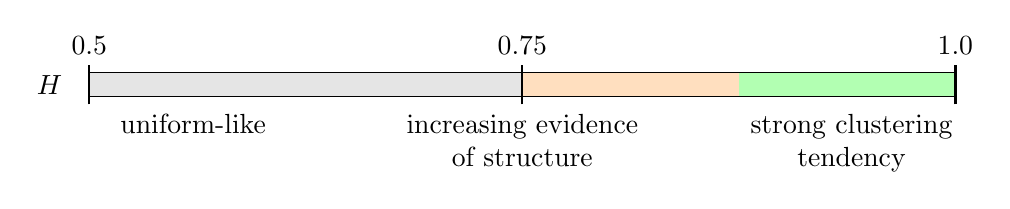
\begin{tikzpicture}[x=22cm]
  \fill[gray!20]   (0.5,0)  rectangle (0.75,0.3);
  \fill[orange!25] (0.75,0) rectangle (0.875,0.3);
  \fill[green!30]  (0.875,0) rectangle (1,0.3);
  \draw (0.5,0) rectangle (1,0.3);
  \foreach \v/\l in {0.5/0.5, 0.75/0.75, 1/1.0}
    \draw[thick] (\v,-0.1) -- (\v,0.4) node[above] {$\l$};
  \node[below, align=center] at (0.56,-0.1) {uniform-like};
  \node[below, align=center] at (0.75,-0.1) {increasing evidence\\of structure};
  \node[below, align=center] at (0.94,-0.1) {strong clustering\\tendency};
  \node[left] at (0.49,0.15) {$H$};
\end{tikzpicture}
\end{center}

\begin{itemize}
  \item $H \approx 0.5$: the data behave similarly to a uniform random distribution.
  \item $H$ increases: random points are farther from the data than sampled data points are from one another.
  \item Rule of thumb: $H > 0.75$ indicates a clear clustering tendency.
\end{itemize}
In terms of hypothesis testing, $H_0$: $D$ is uniformly distributed (no meaningful clusters), $H_1$: $D$ is not uniformly distributed. The statistic is a quick check for clustering tendency, not a clustering algorithm.

\subsection{Partitioning algorithms}

The first thing we need to do is decide how many clusters we want to obtain, $k$. We then cut the data into $k$ distinct groups and choose a representative for each group:
\begin{itemize}
  \item \g{Centroid-based}: the representative is the mean of the points. Efficient and widely used for continuous features.
  \item \g{Medoid-based}: the representative is an observed object. More interpretable and works with arbitrary dissimilarities.
\end{itemize}

\subsubsection{k-means}

In the \g{k-means} algorithm we follow a simple procedure: assign points, update centroids, repeat.

First of all we need an initialization phase where we arbitrarily choose $k$ objects from the dataset as initial centroids $c_i$. We then follow these three steps:
\begin{enumerate}
  \item \s{Assign}: send each point to the nearest centroid $c_i$.
  \item \s{Update}: replace each centroid $c_i$ by the mean of its assigned points,
  \[
    c_i = \frac{1}{|C_i|} \sum_{p \in C_i} p.
  \]
  \item \s{Repeat}: stop when the assignments do not change or the improvement is tiny.
\end{enumerate}
The objective is to minimize the total squared distance to the cluster centroids:
\[
  E = \sum_{i=1}^{k} \sum_{o \in C_i} \norm{o - c_i}^2.
\]
The mean is optimal only for the squared Euclidean distance in a continuous vector space. K-means is fast because each step is easy, but it is not guaranteed to find the global optimum.

K-means is still widely used because it is usually fast and scalable: the complexity is $O(tkn)$, where $t$ is the number of iterations, so it is linear in the number of points. It is also easy to interpret and useful as a summarization tool.

The limitations of k-means and the current fixes are:
\begin{center}
\begin{tabular}{@{}p{4.2cm}p{11cm}@{}}
\toprule
Limitation & Fix \\
\midrule
Sensitive to initialization & Run several restarts; use k-means++ initialization. \\
Sensitive to scale & Standardize variables; choose features and weights carefully. \\
Sensitive to outliers & Trim outliers, use robust preprocessing, or switch to medoids. \\
Assumes convex clusters & For arbitrary shapes, use density-based or graph-based clustering. \\
Requires $k$ & Use the elbow as a diagnostic; validate with silhouette, stability or domain knowledge. \\
Numerical features only & For categorical or mixed data, consider k-modes, k-prototypes or medoids with an appropriate dissimilarity. \\
\bottomrule
\end{tabular}
\end{center}

Another problem in k-means is of course choosing $k$. One of the most popular methods is the heuristic known as the \g{elbow method}: we iteratively increase $k$ starting from one, and for each $k$ we compute the error $E$. If we plot the value of the error we will find an elbow in the curve, and that will be our $k$.

\begin{center}
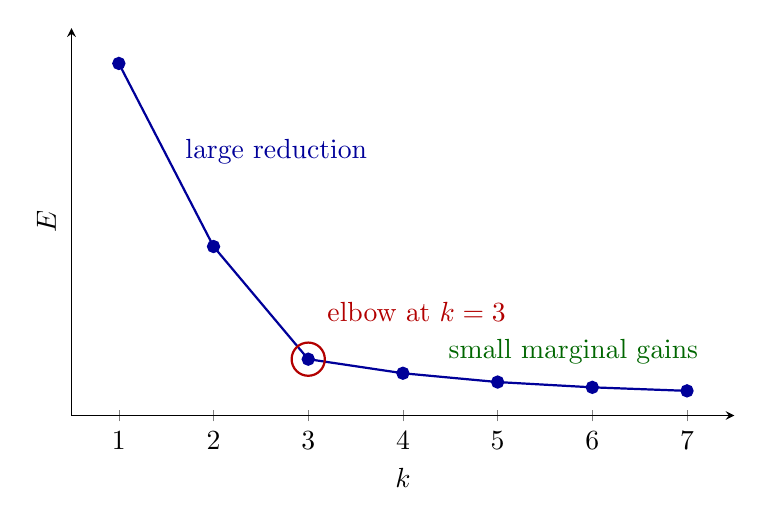
\begin{tikzpicture}
\begin{axis}[
  width=10cm, height=6.5cm,
  xmin=0.5, xmax=7.5, ymin=0, ymax=110,
  xlabel={$k$}, ylabel={$E$},
  xtick={1,...,7}, ytick=\empty,
  axis lines=left, clip=false]
  \addplot[thick, blue!60!black, mark=*] coordinates {(1,100) (2,48) (3,16) (4,12) (5,9.5) (6,8) (7,7)};
  \addplot[only marks, mark=o, mark size=6pt, red!70!black, thick] coordinates {(3,16)};
  \node[above right, red!70!black] at (axis cs:3.1,24) {elbow at $k = 3$};
  \node[right, blue!60!black] at (axis cs:1.6,75) {large reduction};
  \node[above, green!40!black] at (axis cs:5.8,12) {small marginal gains};
\end{axis}
\end{tikzpicture}
\end{center}

The key idea is that we choose the smallest $k$ after which the error decreases only slowly. We don't want to simply minimize the error, because its lower bound is $0$, reached when $k$ is equal to the number of points: increasing $k$ will always reduce the error, but it doesn't mean that the clustering is better. That's why we look for the elbow and not for the minimum.

\subsubsection{k-medoids}

One aspect of k-means we need to have clear is that it is sensitive to outliers: this derives from the fact that we compute the average to choose the centroid. To prevent this we can use the \g{medoid} instead: the medoid is the most central object of the cluster, i.e.\ the real object that minimizes the total dissimilarity to the other objects of the cluster. A single extreme point cannot pull a medoid away like it can pull a mean, so the medoid is much more robust to outliers.

\begin{remark}
The medoid is not the median. The median is computed attribute by attribute and, with more than one attribute, it is in general not an object of the dataset; the medoid is always an observed object. The two coincide only in special cases (e.g.\ one-dimensional data with an odd number of points).
\end{remark}

For the \g{k-medoids} method we can follow the same steps as k-means; the difference is that we don't compute a synthetic representative: we can only move the medoid from a real instance to another real one. This leads to a slower algorithm, because in the worst case we need to try all the points as medoids.

In the literature we have a lot of k-medoids algorithms. They all share the same objective, what changes is the search strategy and its scalability:
\begin{itemize}
  \item \g{PAM / FasterPAM}: exact local-search idea, try the swaps that reduce the total dissimilarity. Modern variants are much faster but still need many distances. Suited for small or medium $n$.
  \item \g{CLARA} (sampling): run k-medoids on samples, then evaluate the medoids on the full data. Useful for large $n$ when a representative sample exists.
  \item \g{CLARANS} (randomized search): explore a random subset of swaps instead of all the neighbors. Suited for a large search space.
  \item \g{BanditPAM} (approximations): use adaptive sampling or approximate distance evaluation to reduce the object-pair checks. Suited for very large $n$.
\end{itemize}

\g{PAM} (Partitioning Around Medoids) works in two phases. The \s{BUILD} phase chooses a useful starting set with a greedy initialization:
\begin{enumerate}
  \item \s{Choose the first medoid}: test every object as the sole representative and keep the one with the smallest sum of distances to all objects,
  \[
    m_1 = \argmin_{h} \sum_{i} d(x_i, h).
  \]
  \item \s{Add one medoid at a time}: for each non-medoid $h$, measure how much it improves the current nearest-medoid distances,
  \[
    gain(h) = \sum_{i} \max\{0,\, D_i - d(x_i, h)\},
  \]
  where $D_i$ is the distance from $x_i$ to its current nearest medoid, and add the candidate with the largest gain.
\end{enumerate}
BUILD is a strong initialization, not a guarantee of the global optimum: PAM still needs the SWAP phase.

The \s{SWAP} phase improves one representative at a time. A neighbor solution replaces one current medoid with one non-medoid:
\begin{enumerate}
  \item \s{Assign}: store each object's nearest current medoid and the total cost $T$.
  \item \s{Evaluate}: for every medoid $m$ and non-medoid $h$, compute the change of cost $\Delta(m \to h)$.
  \item \s{Update}: perform the swap with the most negative $\Delta$, then reassign the objects.
  \item \s{Stop}: if every candidate swap has $\Delta \ge 0$, the solution is a local optimum.
\end{enumerate}
PAM examines the full one-swap neighborhood, but it can still stop at a local, not global, minimum.

The other algorithms reduce the cost of this search in different ways:
\begin{itemize}
  \item \g{CLARA} scales PAM by sampling the objects: it runs BUILD and SWAP only within a small sample, scores the resulting medoids on the full dataset, and repeats for several samples keeping the medoids with the lowest full-data cost. The main risk is that a good medoid, or a small rare cluster, cannot be discovered if it is absent from every sample.
  \item \g{CLARANS} samples the search neighborhood, not the data: it proposes a random swap, moves immediately when the cost improves, and after a chosen number of failed random swaps treats the current solution as a local minimum; then it restarts from another random medoid set and keeps the best local minimum found.
  \item \g{BanditPAM} samples the distance evaluations adaptively: candidates are treated like competing arms, their average cost is estimated from a growing subset of distances, and a candidate is discarded as soon as its optimistic bound is worse than another candidate's pessimistic bound.
\end{itemize}

To decide between k-means and k-medoids we choose the representative that matches the data and the goal:
\begin{itemize}
  \item \s{Use k-means when} data are numerical, scaled, large, and clusters are expected to be compact around average profiles.
  \item \s{Use k-medoids when} representatives must be actual objects, outliers matter, or the distance is not Euclidean.
  \item \s{Use something else when} clusters are non-convex, density varies strongly, or the number of clusters is not naturally fixed.
\end{itemize}

\begin{center}
\begin{tabular}{@{}lcc@{}}
\toprule
 & k-means & k-medoids \\
\midrule
Speed on vectors & high & medium \\
Robustness to outliers & low & high \\
Interpretability of the representative & medium & high \\
Arbitrary distances & low & high \\
\bottomrule
\end{tabular}
\end{center}
